% !TEX root = template.tex

\section{Taxonomy}

To understand the taxonomic distribution of proteins within our family, we utilized a systematic approach to collect and analyze lineage data for the $83$ sequences found in our family. Using the protein identifiers obtained from PSI-BLAST~\cite{psiblast} and HMM-SEARCH~\cite{hmmer}, we queried the UniProt API~\cite{uniprot_api} to fetch the complete taxonomic lineage for each protein. This process captured the hierarchical classification of each protein within its biological domain, from the broadest category (e.g., \textit{Eukaryota}) to the most specific organism classification, and allowed for representation using the Newick tree format~\cite{newick_format} (Fig.~\ref{fig:phylo-tree}). Several interesting patterns can be observed in the graph.

The collected lineage data was then processed to calculate frequency counts for each taxonomic level. By traversing the hierarchical taxonomy, we were able to generate a nested dictionary representing the occurrence of each taxonomic node across the dataset. This allowed for a detailed visualization of taxonomic diversity.

The taxonomic tree was plotted using the ETE Toolkit~\cite{ete_toolkit}, leveraging the Newick format derived from the hierarchical data. Node sizes in the phylogenetic tree were adjusted to reflect the relative abundance of each taxonomic entity, with larger nodes indicating higher representation in the protein family. (Fig.~\ref{fig:phylo-tree}) Illustrates the resulting phylogenetic tree, showcasing the distribution of proteins across various taxonomic groups. Notable clusters include a strong representation within mammals, particularly in the order \textit{Primates}, as well as significant diversity within arthropods.


\begin{figure*}[h!]
    \centering
    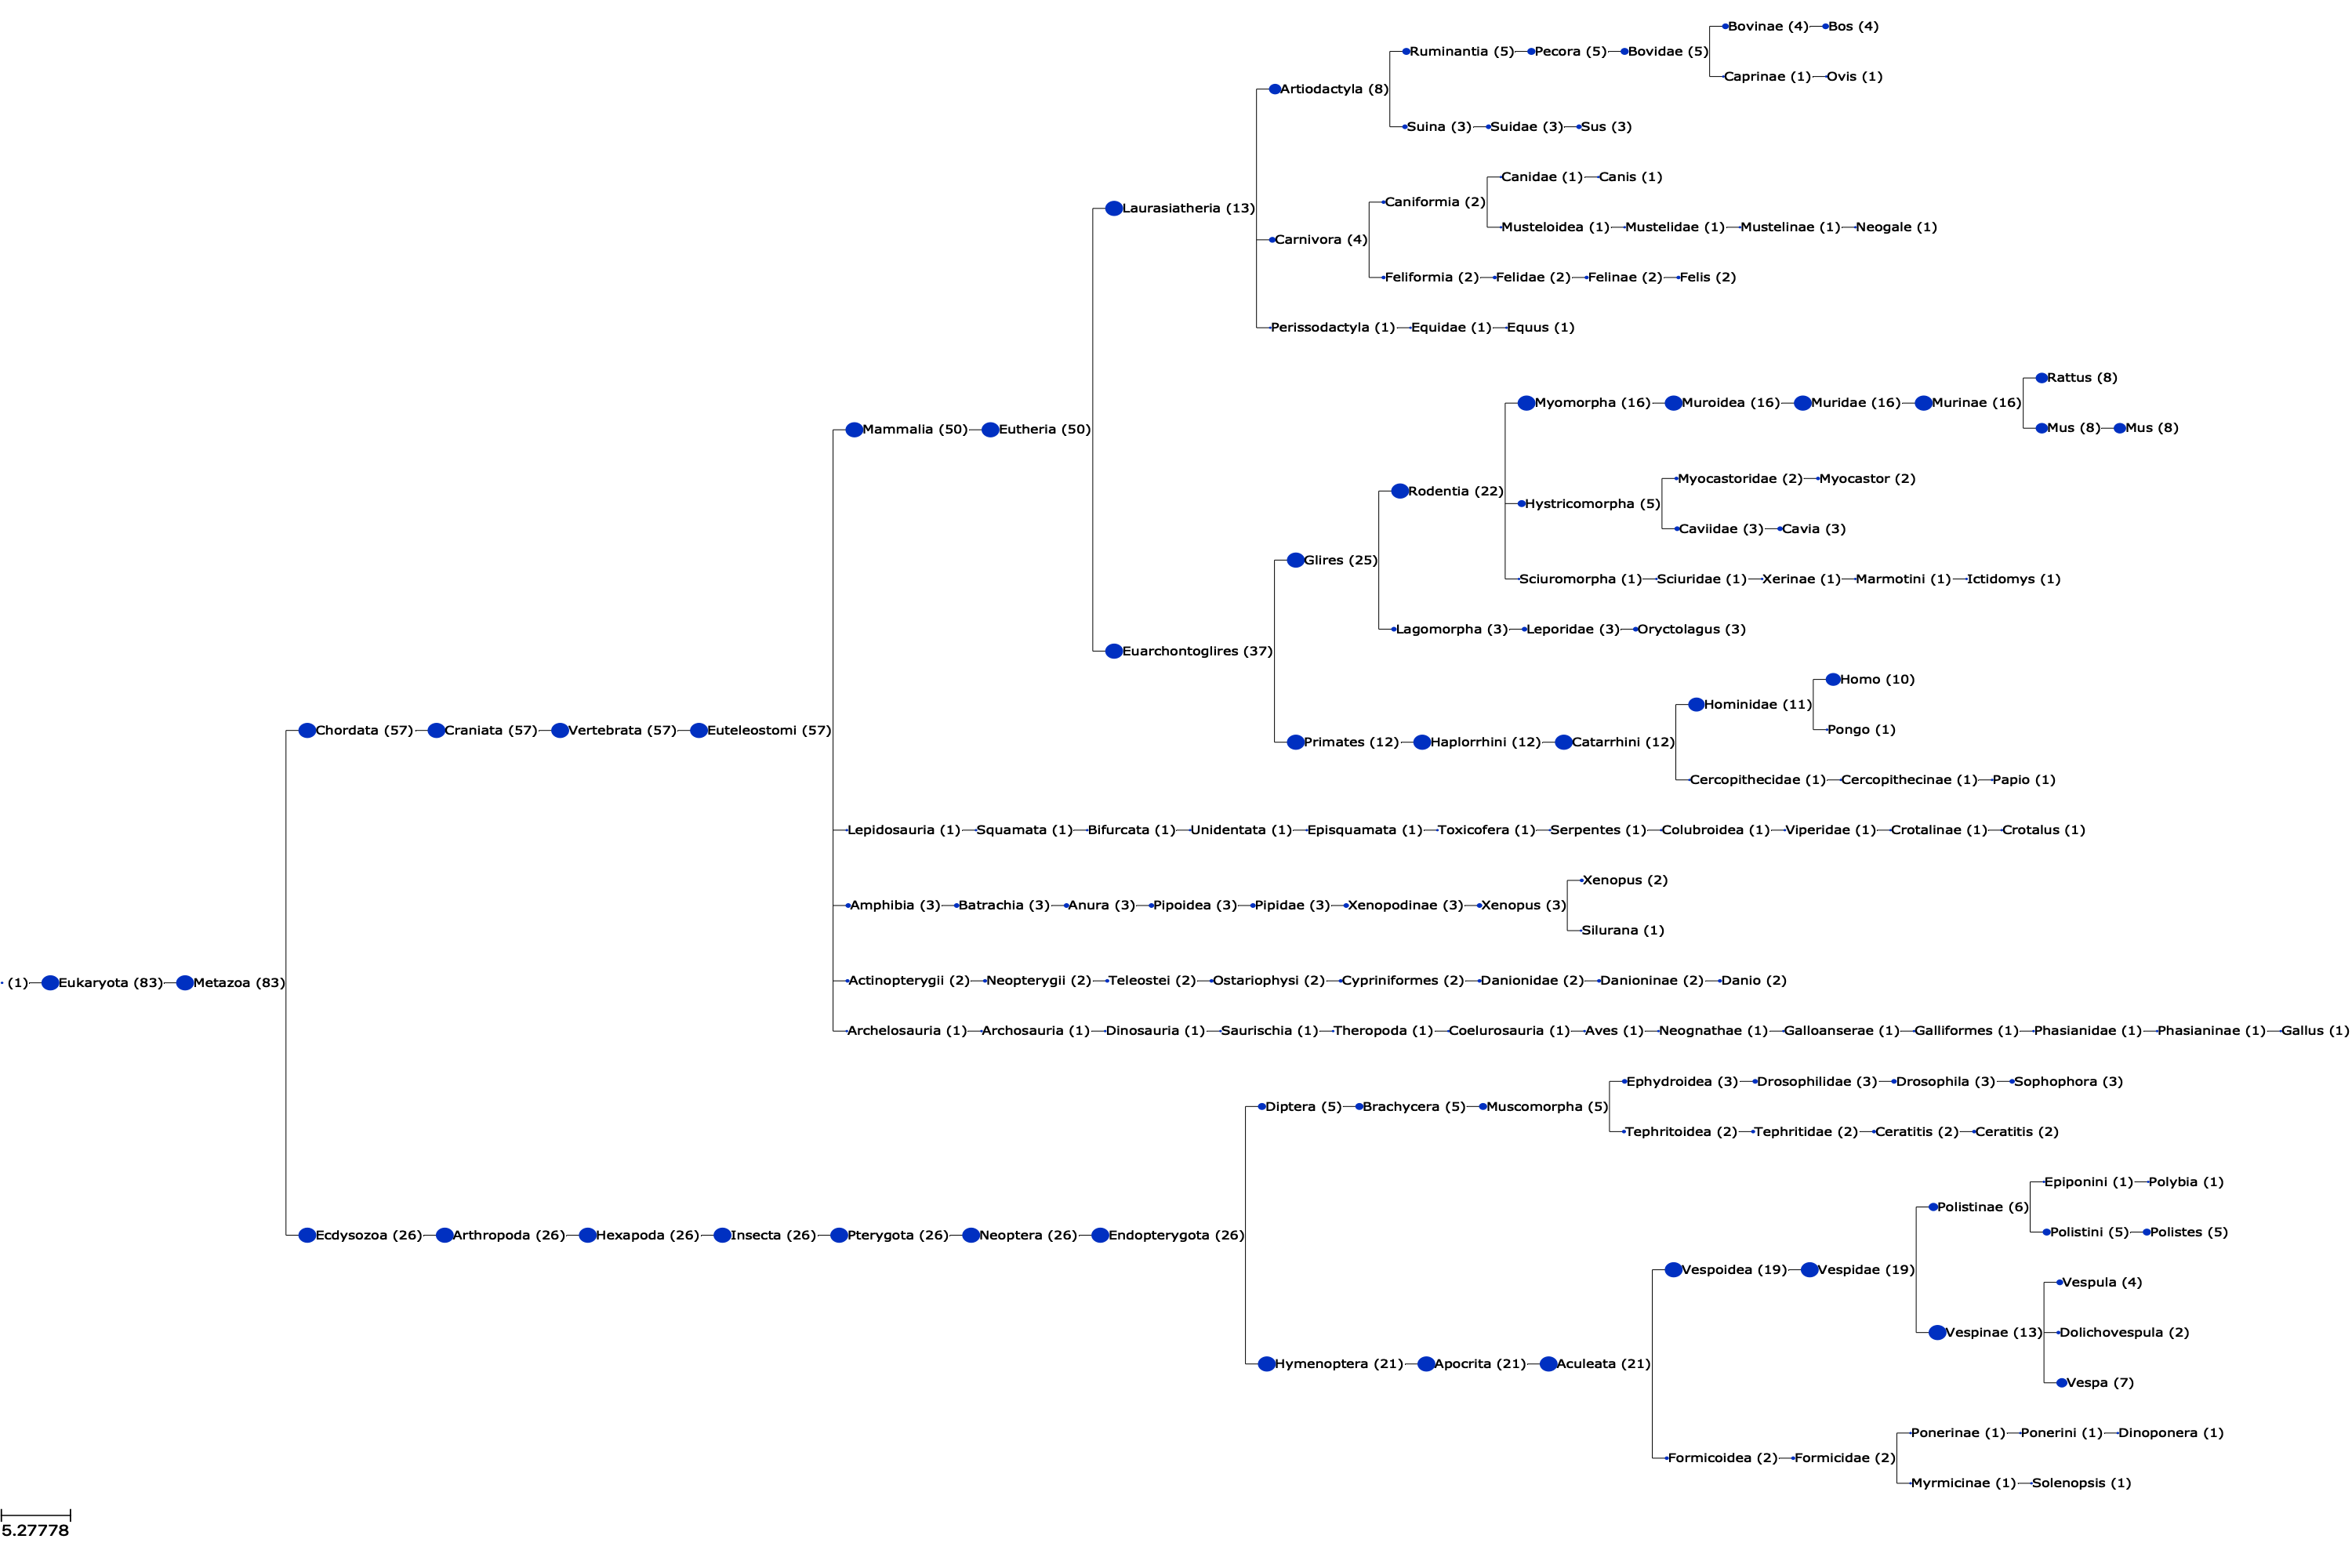
\includegraphics[width=0.8\textwidth]{images/phylogenetic_tree_freq.png}
    \caption{Phylogenetic tree illustrating taxonomic relationships across family sequences, with node sizes reflecting relative abundance. The tree highlights a dominant presence in mammals, particularly \textit{Primates}, and significant diversity within arthropods. This visualization underscores the evolutionary adaptation and taxonomic distribution of the protein domain.}
    \label{fig:phylo-tree}
\end{figure*}